%\documentclass[handout]{beamer}\mode<presentation>{\usetheme{AMSCesenaPurpleAndGold}}
\documentclass[presentation]{beamer}\mode<presentation>{\usetheme{AMSCesenaPurpleAndGold}}
%%%%

\usepackage{sd-lab-building-linda}
\usepackage{my-listings}
\usepackage{forloop}

\title[L3 -- Building \linda{}]{Building \linda{} from scratch}
%
\subtitle[SD]
{Distributed Systems / Hands-on\\\scriptsize Sistemi Distribuiti / Laboratorio}
%
\author[Ciatto \and Omicini]
{\emph{Giovanni Ciatto} \and Andrea Omicini\\
	\texttt{giovanni.ciatto@unibo.it} \and \texttt{andrea.omicini@unibo.it}}
%
\institute[DISI, Univ. Bologna]
{Dipartimento di Informatica -- Scienza e Ingegneria (DISI)\\\textsc{Alma Mater Studiorum} -- Universit{\`a} di Bologna a Cesena}
%
\date[A.Y. 2019/2020]{Academic Year 2019/2020}

\setbeamercovered{transparent}

\begin{document}
	
%\\\\\\\\\\\\\\\\\\\\\
\frame{\titlepage}
%\\\\\\\\\\\\\\\\\\\\\

\section{Wetting your appetite}

\begin{frame}
\frametitle{Motivation \& Lecture Goals}

\begin{itemize}
	\item
\end{itemize}

\end{frame}

\begin{frame}
\frametitle{Lab 3 Repository on GitLab}

	\begin{itemize}
		\item Examples and exercises described in this lecture are provided by means of the following GitLab repository:
		%
		\begin{center}
			\url{https://gitlab.com/pika-lab/courses/ds/aa1920/lab-04}
		\end{center}
		
		\vfill
		
		\item Clone it on your machine using Git
		%
		\begin{itemize}
		    \item[\$] \texttt{git clone \textit{<repo URL>}}
		\end{itemize}
		
		\vfill
		
		\item Even if a minimal environment simply relying on a text editor + Gradle is sufficient for this lab, we kindly suggest to import the cloned repository into some IDE, e.g. IntelliJ Idea or Eclipse
		%
		%
		\begin{itemize}
		    \item in case of problems in importing the project on IntelliJ, try to downgrade the gradle wrapper
		    %
		    \item[\$] \texttt{./gradlew wrapper \alert{--gradle-version \textit{4.8.1}}}
		\end{itemize}
		
		\vfill
		
		\item In order to be able to submit your exercises, please ensure you requested access to the \href{https://gitlab.com/pika-lab/courses/ds/aa1920}{GitLab group of the course}
	\end{itemize}

\end{frame}

\section{Linda Recap}

\subsection{Overview} 

\begin{frame}%[allowframebreaks]
\frametitle{The \linda{} model}

\begin{itemize}
	\item<1-> The \linda{} model is built up of five main (sorts of) elements:
	%
	%
	\begin{description}
		\item[Tuples] | structured information chunks (such as strings, records, dictionaries, or other kinds of \alert{data structures})
		
		\item[Templates] | compact notations for expressing sets of tuples adhering to the same pattern (e.g. regular expressions are templates w.r.t. strings).
		%
		Such patterns express some \alert{partial knowledge} about one or more tuple
		
		\item[Tuple Spaces] | unordered containers (i.e., \alert{multisets}) of tuples, which may evolve over time since tuples may be added or removed
		
		\item[Agents] (or ``Processes'', or ``Activities'') | pro-active entities which interact by writing, observing, or taking information from the tuple spaces
		
		\item[Primitives] | operations which can be performed by agents on tuple spaces, in order to manipulate or observe the information they contain
		
	\end{description}
	
\end{itemize}

\end{frame}

\subsection{Primitives} 

\begin{frame}%[allowframebreaks]
\frametitle{\linda{'s} primitives}

\begin{itemize}
\item The minimal set of \alert{primitives} according to the original \linda{'s} model comprehends the following ones:
%

%
\begin{description}
	\item[\texttt{out}] | let agents \alert{write} (or \alert{insert}) a tuple into a tuple space 
	
	
	
	\item[\texttt{rd}] (shortcut for \alert{read}) | let agents know if a tuple matching a particular template \alert{exists} on a tuple space. 
	%
	If it is the case, agents can also read the content of such a tuple
	
	
	
	\item[\texttt{in}] | let agents \alert{take} (or \alert{consume}) a tuple matching a particular template on a tuple space, if any
\end{description}



\item Other primitives will be considered in the future, but for the moment this is all we need



\item Think about tuple spaces as \alert{collections}, about tuples as the the elements contained by such collections, and about primitives as the \alert{interface} of tuple spaces

\end{itemize}

\end{frame}

\subsection{The blackboard metaphor} 

\begin{frame}
\frametitle{The blackboard metaphor}

\begin{enumerate}
\item You can imagine a tuple space as a \alert{blackboard}
%
\begin{center}
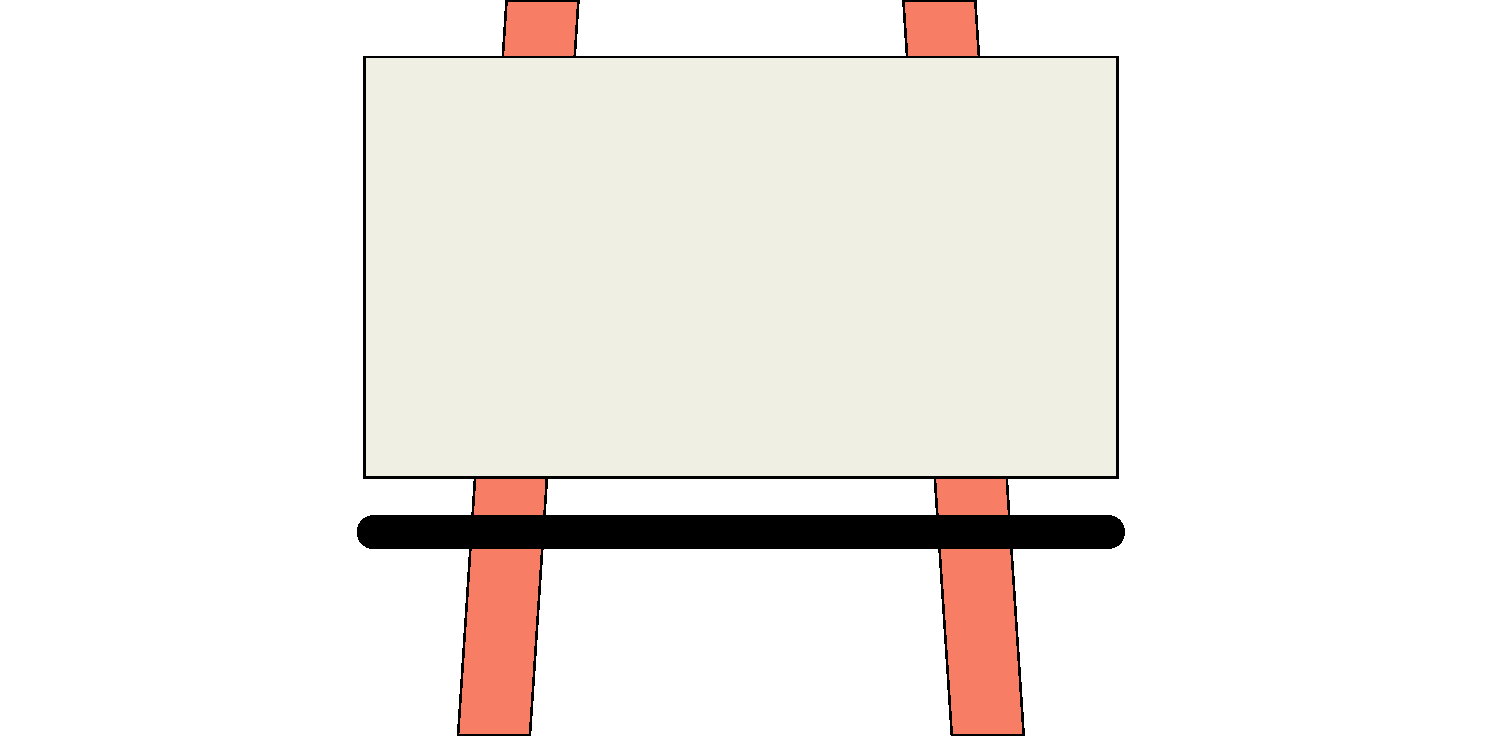
\includegraphics[width=\linewidth]{./img/blackboard.pdf}
\end{center}
%
\end{enumerate}

\end{frame}

\newcounter{imagenumber}

\forloop{imagenumber}{1}{\value{imagenumber} < 4}{
\begin{frame}
\frametitle{The blackboard metaphor}

\begin{enumerate}\setcounter{enumi}{2}
    \item where agents can \alert{\texttt{write}} any sort of information---[i.e.] \alert{tuples}
    \begin{itemize}
        \item according to some \alert{representation} format of choice 
        \item through primitive \alert{\texttt{out}}
    \end{itemize}
%
\begin{center}
\includegraphics[width=\linewidth]{./img/write-\arabic{imagenumber}.pdf}
\end{center}
%
\end{enumerate}

\end{frame}
}

\forloop{imagenumber}{1}{\value{imagenumber} < 4}{
\begin{frame}
\frametitle{The blackboard metaphor}

\begin{enumerate}\setcounter{enumi}{3}

\item where agents can \alert{\texttt{read}} all information matching a particular \alert{template}
    \begin{itemize}
        \item according to some \alert{query} language of choice 
        \item through primitive \alert{\texttt{rd}}
    \end{itemize}
%
\begin{center}
\includegraphics[width=\linewidth]{./img/read-\arabic{imagenumber}.pdf}
\end{center}
%
\end{enumerate}
\end{frame}
}

\forloop{imagenumber}{1}{\value{imagenumber} < 4}{
\begin{frame}
\frametitle{The blackboard metaphor}

\begin{enumerate}\setcounter{enumi}{4}

\item or \alert{\texttt{take}} it, making it unaccessible for other agents
%
\begin{itemize}
    \item through primitive \alert{\texttt{in}}
\end{itemize}
%
\begin{center}
\includegraphics[width=\linewidth]{./img/take-\arabic{imagenumber}.pdf}
\end{center}
\end{enumerate}
\end{frame}
}

\subsection{Semantics} 

\begin{frame}%[allowframebreaks]
\frametitle{(Semi-)Formal notation}

In what follows, we will use the following notation:
%
\vfill
%
\begin{itemize}
\item Tuples are enumerated by \alert{$t$}, or $t_i$, so, for instance, $t_1 \neq t_2$, but $t_0 = t_0$

\item Templates are enumerated by \alert{$\bar{t}$}, or $\bar{t}_i$. Notice that templates are a compact way to represent \alert{sets} of tuples

\item Matching is written as \alert{$t \in \bar{t}$}, i.e., tuple $t$ matches template $\bar{t}$
%
\begin{itemize}
\item unless stated otherwise, we implicitly assume the following notation: tuple $t$ matches template $\bar{t}$, tuple $t_1$ matches template $\bar{t_2}$, tuple $t_i$ matches template $\bar{t_i}$, and so on \ldots
\end{itemize}

\item Tuple Spaces are enumerated by \alert{$TS$}, or $TS_j$

\item Agents are enumerated by \alert{$A$}, or $A_k$
\end{itemize}

\end{frame}

\begin{frame}[fragile]
\frametitle{\linda{'s} semantics}
\label{linda-semantics}

\begin{description}
\item[Generative] | after an agent $A$ performs a \texttt{out($t$)} operation on some tuple space $TS$, tuple $t$ \alert{exists} regardless of $A$. 
%
If agent $A$ terminates, crashes, or disconnects, $t$ will keep existing on $TS$

\item[Associative] | tuples are \alert{accessed} (read or taken) in an associative way: instead of using a name, or an address, agents can specify \alert{templates} in order to access tuples

\item[Suspensive] | whenever an agent $A$ invokes the \texttt{rd($\bar{t}$)} or \texttt{in($\bar{t}$)} over a particular template $\bar{t}$, on a particular tuple space $TS$, if not tuple $t$ matching $\bar{t}$ exists on $TS$, the operation is \alert{suspended} until $t$ is inserted into $TS$ by some agent performing a \texttt{write($t$)} operation

\item[Non-deterministic] | whenever an agent $A$ invokes the \texttt{read($\bar{t}$)} or \texttt{take($\bar{t}$)} operation, if more than one tuple $t$, $t'$, $t''$ exist matching  $\bar{t}$, one is retrieved \alert{non-deterministically}

\end{description}

\end{frame}


\section{Implementing \linda{} in Java}

\subsection{Design} 

\begin{frame}%[allowframebreaks]
\frametitle{\linda{} as a Java interface}

\begin{itemize}
	\item A tuple space can be easily conceived as an \alert{object} in the OOP sense
	
	\vfill
	
	\item But how should control-flow related aspects be faces?
\end{itemize}

\vfill

\lstinputlisting{./code/TupleSpace.java}

\vfill

\begin{itemize}
	\item Where \texttt{Future<X>} is the return type for \alert{asynchronous} operations
	%
	\begin{itemize}
		\item its functioning will be clear in a few slides
	\end{itemize}
\end{itemize}
\end{frame}

\subsection{Tuples \& Templates interfaces} 

\begin{frame}%[allowframebreaks]
\frametitle{Where \texttt{Tuple}s and and \texttt{Template}s are simply:}

\columnsHH{
\lstinputlisting{./code/Tuple.java}
}{
\lstinputlisting{./code/Template.java}
}

\begin{itemize}
\item Tuples may be potentially anything



\item Templates may be anything able to match a tuple, somehow
\end{itemize}

\vfill

\begin{block}{Of course, this is just an abstract model}
How should we \alert{actually} implement it?
\end{block}

\end{frame}

\subsection{Text-based Tuple Spaces in Java}

\begin{frame}%[allowframebreaks]
\frametitle{Text-based Tuple Spaces in Java, idea}

We will implement the \texttt{TupleSpace} interface by means of the \texttt{\alert{Text}TupleSpace} class, where:
%
\vfill
%
\begin{itemize}
\item Strings are used as tuples, meaning that the \texttt{java.lang.\alert{String}} class is used to reify tuples
%
\begin{itemize}
\item[i.e.] \texttt{T = String}
\end{itemize}



\item Regular Expressions (regex) are used as templates, meaning that the \texttt{java.util.regex.\alert{Pattern}} class is used to reify templates
%
\begin{itemize}
\item[i.e.] \texttt{TT = Pattern}
\end{itemize}



\item The matching consists of \alert{deciding} whether a string matches a regex

\vfill

\item[!] If you are not practical with regex, you can acquire some experience or simply test your patterns with \url{https://regex101.com}
\end{itemize}

\end{frame}

\begin{frame}
\frametitle{String as Tuples}

\lstinputlisting{./code/StringTuple.java}
%
\end{frame}

\begin{frame}
\frametitle{Regex as Templates}

\lstinputlisting{./code/RegexTemplate.java}

\end{frame}

\begin{frame}
\frametitle{\href{https://regex101.com/}{Regex101.com} -- Example}

\begin{itemize}
\item Could you say what's the meaning of the following regex?
%
\begin{center}
\small\alert{
\texttt{to:\,\textbackslash{}"([A-Za-z ]+)\textbackslash{}",\,from:\,\textbackslash{}"([A-Za-z ]+)\textbackslash{}",\,content:\,\textbackslash{}"(.*?)\textbackslash{}"}}
\end{center}
%

%
\begin{center}
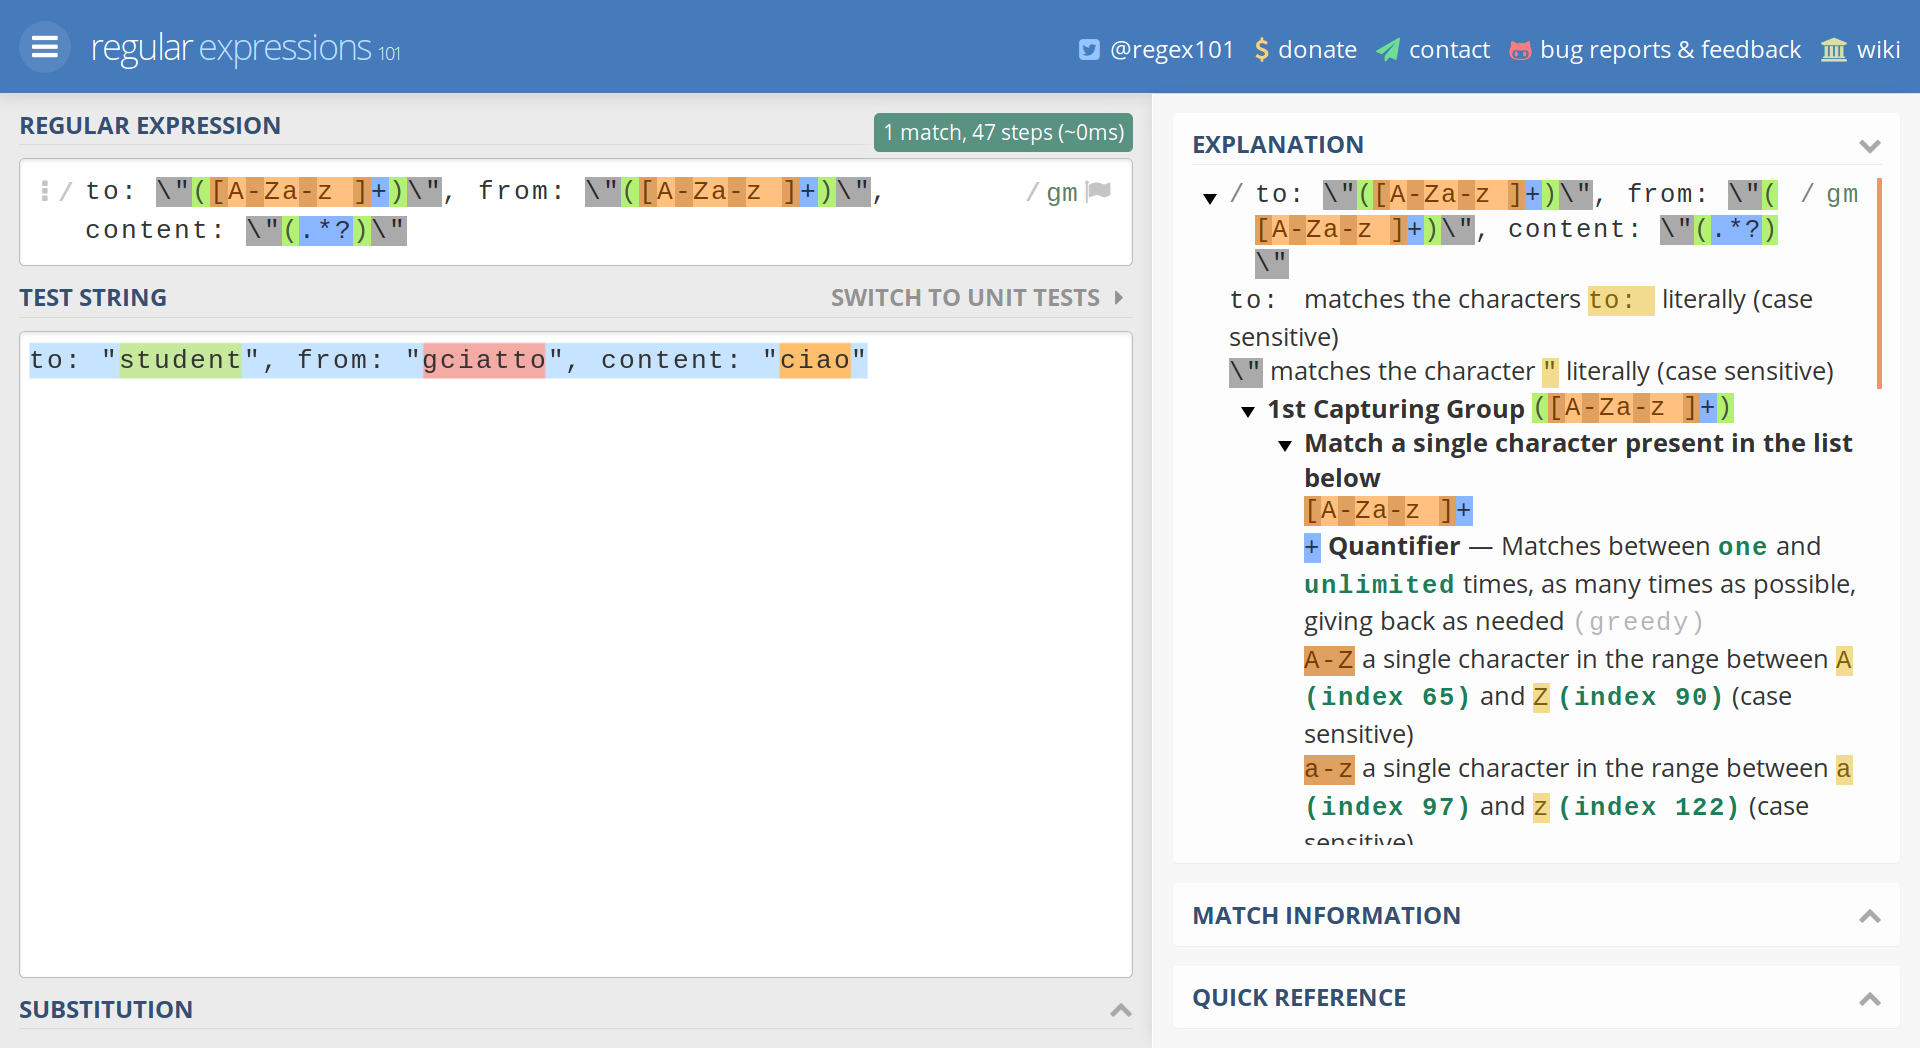
\includegraphics[width=.7\linewidth]{./img/regex101.png}
\end{center}

\item \url{https://regex101.com} provides an interactive explaination of your regex (on the right side) 

\item you can test your regex on the fly against any input string

\end{itemize}  
\end{frame}

\subsection{Exercise 3-1} 

\begin{frame}[allowframebreaks]
\frametitle{Exercise 3-1: Text-based Tuple Spaces in Java}

\begin{enumerate}
	\item Clone the initial source code from \url{https://gitlab.com/das-lab/courses/ds/aa1819/lab-3}
	
	\item Import the project into your favourite IDE as a Gradle project
	
	\item Inspect the project and try to figure out the purpose of the provided code
	
	\item Notice that the project's \texttt{build.gradle} file comes with some dependencies.
	%
	Try to figure out what they are and what's their purpose
	
	\item Notice that the project comes equipped with some tests. 
	%
	Read them and try to understand them
\end{enumerate}

\lstinputlisting{./code/TextTupleSpace.java}

\framebreak

Your solution must satisfy the following constraints:
%
\begin{itemize}
	
	\item The \alert{unit tests} contained within the \alert{\texttt{TestTextTupleSpace}} class must be satisfied
	%
	\begin{itemize}
		\item use them usage as examples
		\item consider looking at the other \texttt{Test*} classes, in order to understand how Executor Services or Futures work
	\end{itemize}
	
	\item You \alert{shouldn't need any threads}, just use Executor Services and Active Objects (to act as Agents)
	
	\item The tuple space must work regardless of the particular Executor Service it is initialised with
	
	\item The provided implementation must adhere to the \alert{\linda{} semantics} described on slide \ref{linda-semantics}
	
	\vspace{.3 cm}
	
	\item[!] If you feel confident with these concepts you can start your exercise now. 
	%
	Otherwise, just wait for the teacher's tutorial
\end{itemize}

\framebreak

While solving your exercise on your branch:
%
\vspace{.3cm}
%
\begin{alertblock}{It is strictly \textbf{forbidden}}
	\begin{itemize}
		\item to alter, remove, ignore, or comment the \alert{\texttt{.gitlab-ci.yml}} file on your branch
		\item to alter, remove, ignore, or comment the provided test classes
		\item[!] submissions subject to such kind of problems will be considered \alert{late}
	\end{itemize}
\end{alertblock}
%
\vspace{.3cm}
%
\begin{exampleblock}{If you understand some test is faulty or ill-constructed}
	\begin{itemize}
		\item you \alert{must} post the information on the forum \alert{as soon as possible}
	\end{itemize}
\end{exampleblock}
\end{frame}

%===============================================================================
\section*{}
%===============================================================================

%\\\\\\\\\\\\\\\\\\\\\
\frame{\titlepage}
%\\\\\\\\\\\\\\\\\\\\\

%%===============================================================================
%\section*{\refname}
%%===============================================================================
%
%%\\\\\\\\\\\\\\\\\\\\\
%%%%%
%%\begin{frame}[t,allowframebreaks]\scriptsize
%\begin{frame}[c]\footnotesize
%\frametitle{\refname}
%\bibliographystyle{apalike}
%\bibliography{sd-lab-building-linda}
%\end{frame}
%%\\\\\\\\\\\\\\\\\\\\\

%%%%%%%%%%%%%%%%%%%%%%%%%%%%%%%%%%%%%%%%%%%%%%%%%%%%%%%%%%%%%%%%%%%%%%%%%%%%%%%
\end{document}
%%%%%%%%%%%%%%%%%%%%%%%%%%%%%%%%%%%%%%%%%%%%%%%%%%%%%%%%%%%%%%%%%%%%%%%%%%%%%%%%

